\documentclass[11pt,letterpaper]{article}
\usepackage[utf8]{inputenc} %Codificacion del texto (ISO Latin1 encoding)

\usepackage{fancyhdr} %Permite acomodar a tu gusto la parte de arriba y
% abajo del documento
\usepackage[spanish]{babel} %Permite definir el idioma del dcumento
\usepackage{graphicx} %Permite exportar imagenes en formato eps
\usepackage{url} %Tipo de fuente para correos y paginas
\usepackage{pgf}
\usepackage{fleqn}
\usepackage{amssymb}
\usepackage{fancyvrb}
\usepackage{sectsty}
\usepackage{makeidx}
\usepackage{colortbl} %Permite colocar colores a las tablas
\usepackage{booktabs}
%%%%%%%%%%
%Margenes%
%%%%%%%%%%
\parskip 1mm %Espacio entre parrafos

\setlength{\topmargin}{0pt}

\oddsidemargin	0.5cm  % Ancho Letter 21,59cm
\evensidemargin 0.5cm  % Alto  Letter 27,81cm
\textwidth	15.5cm
\textheight	21.0cm
\headsep	4 mm
\parindent	0.5cm
%%%%%%%%%%%%%%%%%%%%%%
%Estilo del documento%
%%%%%%%%%%%%%%%%%%%%%%
\pagestyle{fancyplain}

%%%%%%%%%%%%%%%%%%%%%%%%%%%%%%%%%%%%%%%%%%%
%Fancyheadings. Top y Bottom del documento%
%%%%%%%%%%%%%%%%%%%%%%%%%%%%%%%%%%%%%%%%%%%
% Recuerde que en este documento la portada del documento no posee
% numeracion, pero de igual manera llamaremos a esa primera pagina la numero
% 1, y la que viene la dos. Esto es para tener una idea de las que
% llamaremos pares e impares
\lhead{Sistemas y Organizaciones} %Parte superior izquierda
\rhead{\bf \it Informe 1} %Parte superior derecha
\lfoot{\it Émile Durkheim} %Parte inferior izquierda. \thepage indica
% el numero de pagina
\cfoot{} %Parte inferior central
\rfoot{\bf \thepage} %Parte inferior derecha
\renewcommand{\footrulewidth}{0.4pt} %Linea de separacion inferior

% Challa

\newtheorem{theorem}{Theorem}
\newtheorem{acknowledgement}[theorem]{Acknowledgement}
\newtheorem{algorithm}[theorem]{Algorithm}
\newtheorem{axiom}[theorem]{Axiom}
\newtheorem{case}[theorem]{Case}
\newtheorem{claim}[theorem]{Claim}
\newtheorem{conclusion}[theorem]{Conclusion}
\newtheorem{condition}[theorem]{Condition}
\newtheorem{conjecture}[theorem]{Conjecture}
\newtheorem{corollary}[theorem]{Corollary}
\newtheorem{criterion}[theorem]{Criterion}
\newtheorem{definition}[theorem]{Definition}
\newtheorem{example}[theorem]{Example}
\newtheorem{exercise}[theorem]{Exercise}
\newtheorem{lemma}[theorem]{Lemma}
\newtheorem{notation}[theorem]{Notation}
\newtheorem{problem}[theorem]{Problem}
\newtheorem{proposition}[theorem]{Proposition}
\newtheorem{remark}[theorem]{Remark}
\newtheorem{solution}[theorem]{Solution}
\newtheorem{summary}[theorem]{Summary}
\newenvironment{proof}[1][Proof]{\noindent\textbf{#1.} }{\ \rule{0.5em}{0.5em}}

\newcommand{\primaria}[1]{
	\textbf{\underline{#1}}
}

\newcommand{\foranea}[1]{
	\textbf{\textsl{#1}}
}

\newcommand{\primyfor}[1]{
	\underline{\foranea{#1}}
}

\makeatletter
\newcommand\subsubsubsection{\@startsection {paragraph}{1}{\z@}%
                                   {-3.5ex \@plus -1ex \@minus -.2ex}%
                                   {1.5ex \@plus.2ex}%
                                   {\normalfont\bfseries}}
\newcommand\subsubsubsubsection{\@startsection {subparagraph}{1}{\z@}%
                                   {-3.5ex \@plus -1ex \@minus -.2ex}%
                                   {1.5ex \@plus.2ex}%
                                   {\normalfont\bfseries}}


\makeatother

%\makeindex
%%%%%%%%%%%%%%%%%%%%%%%%%%%%%%%%%%%%%%%%%%%%%%%%%%%%%%%%%%%%%%%%%%%
%%%%%%%%%%%%%%%%%%%% Aqui empieza el documento %%%%%%%%%%%%%%%%%%%%
%%%%%%%%%%%%%%%%%%%%%%%%%%%%%%%%%%%%%%%%%%%%%%%%%%%%%%%%%%%%%%%%%%%

\begin{document}

%%%%%%%%%%%%%%%%%%%%%%%%%%
%Definicion de la portada%
%%%%%%%%%%%%%%%%%%%%%%%%%%
\begin{titlepage}
    \begin{center}
	\begin{tabular}{ccc}
	     
\includegraphics[height=1.9cm]{images/utfsm}
	    & 
	    \hspace{0.2cm}
	    \begin{tabular}{c}
		Universidad Técnica Federico Santa María \\ \hline
		\hspace{8.0cm}
		\vspace{1.2cm}
	    \end{tabular}
	    \hspace{0.2cm}
	    &
            
\includegraphics[height=2cm]{images/di}
	\end{tabular}

	\vspace{1.5cm}
	%Titulo del Documento
	    \begin{tabular}{c}
		\Huge{\textbf{Informe 2}}\\\\
		\LARGE{\sc{Sistemas y Organizaciones}}\\
		\LARGE{\sc{{``Elian y Compañía''}}}
	    \end{tabular}

	\vspace{0.5cm}
	\begin{center}
		\Large{Teorías}\\
		\begin{itemize}
			\small
		        \item \textbf{Luther\ Gullick:} \emph{``PODSCORB''}\\
		        \item \textbf{Adam\ Smith:} \emph{``La Riqueza de las Naciones''}\\
		        \item \textbf{\'Emile\ Durkheim:} \emph{``Hechos sociales''}\\
		        \item \textbf{Frederick\ Taylor:} \emph{``Administración Científica''}
		        \item \textbf{Mary\ Parker\ Follet:} \emph{``El Nuevo Estado''}\\
		        \item \textbf{Chester\ Barnard:} \emph{``Influencia de factores sicológicos y sociales en la efectividad de la organización''}\\
		        \item \textbf{Fred\ Emery:} \emph{``Sistemas Sociotécnicos''}\\
		\end{itemize}

	\end{center}
	
        \vspace{1cm}

	%Nombre del (o los) autor(es)
	\begin{tabular}{cc}
	   \begin{tabular}{c}
         	\large{Rodrigo Fernández - 2673002-3}\\ 
		\large{\url{rfernand@inf.utfsm.cl}}\\
	   \end{tabular}
		&
	   \begin{tabular}{c}
         	\large{Javier Olivares - 2673043-0}\\ 
		\large{\url{jolivaro@inf.utfsm.cl}}
	   \end{tabular}
	\end{tabular}
	   \begin{tabular}{c}
		\\
         	\large{Cristi\'an Maureira - 2673030-9}\\ 
		\large{\url{cmaureir@inf.utfsm.cl}}\\
	   \end{tabular}

	% Nombre profesor asignatura
	\begin{center}
		\large{\textbf{Profesor:} Lautaro Guerra Genskowsky}
	\end{center}

        \vspace{1cm}
	%Fecha
		\large{\sc{\today}}
    \end{center}
\end{titlepage}


\tableofcontents
\newpage

\section{Resumen}
\label{sec:introduccion}
\vspace{1cm}
Por medio del presente informe se desarrollará en profundidad,
el legado del trabajo de \emph{Émile Durkheim}, analizando sus
ideas principales, rescatando así los factores negativos y positivos
de su trabajo.
\vspace{1cm}

Para tener una idea global de la importancia del personaje histórico
analizado a continuación, tenemos que comprender primeramente que es
uno de los fundadores de la sociología moderna, ya que a través de sus
esfuerzos en éste ámbito, se logró comprender con claridad las diferencias
entre la \emph{Sicología} y la \emph{Sociología}.
\vspace{1cm}

Present\'o variadas ideas basadas en el estudio de la sociedad,
entre ellas, vale destacar la del ``trabajo social'' y la idea de ``hechos sociales'', el cual mediante el método científico realizó un estudio a la sociedad, tratando de eliminar el sentimentalismo e ilusionismo, de dicho aspecto.
\vspace{1cm}

Sobre las bases de nuestro trabajo, cambiamos la estructura de los informes entregados anteriormente y los complementamos con mayor detalle,
 adem\'as de aportar con el contexto hist\'orico y filos\'ofico de la \'epoca para poder comprender mejor los antecedentes del trabajo realizado por Durkheim.
 Tambi\'en, agregamos las obras del autor junto con un peque\~no resumen de cada una de ellas.

\newpage



\section{Antecedentes}
\label{sec:contextoHistorico}
\subsection{Contexto Hist\'orico}

\begin{enumerate}
\item \textbf{El\ segundo\ imperio\ de\ Napole\'on}

 Comenz\'o en el plebiscito que proclam\'o emperador a Luis Napole\'on Bonaparte (1852). Su gobierno se apoy\'o en el clero, en la alta burgues\'ia y en la poblaci\'on rural. Sigui\'o una pol\'itica empe\~nada en realzar el prestigio del pa\'is y del r\'egimen; en esa \'epoca, Haussmann embelleci\'o la capital. En pol\'itica exterior se inici\'o la conquista del Senegal, se penetr\'o en Argelia y se intervino en Indochina. Tambi\'en se apoy\'o a Italia en su lucha contra Austria por la unificaci\'on y se impuso a Maximiliano I como emperador de M\'exico (1862-1867). El r\'egimen se basaba en la prosperidad econ\'omica, pero \'esta entr\'o en crisis en 1870 cuando la desastrosa derrota de Sedan en la guerra francoprusiana (1870) puso fin al imperio, proclam\'andose la rep\'ublica.

\item \textbf{La\ tercera\ rep\'ublica}

La comuna revolucionaria de Par\'is, que hab\'ia surgido aprovechando el vac\'io del poder (1871), fue aplastada. Se elabor\'o la constituci\'on de 1875, de car\'acter conservador, como correspond\'ia al miedo de la burgues\'ia tras la revoluci\'on de 1871. Sin embargo, el movimiento obrero obtendr\'ia m\'as tarde la legalizaci\'on de los sindicatos (1884). En 1902 el bloque de izquierdas triunf\'o en las elecciones; se separ\'o la Iglesia del estado (1905), se difundi\'o la ense\~nanza laica y se intent\'o hacer frente a los problemas sociales mediante una legislaci\'on protectora de los trabajadores. En el exterior, durante el per\'iodo 1870-1914 se forj\'o un imperio colonial en \'Africa e Indochina, que fue el segundo en extensi\'on despu\'es del de Gran Breta\~na y mejor\'o la imagen del pa\'is.

La pugna con Alemania, que le hab\'ia arrebatado Alsacia y Lorena (1871), llev\'o a la Entente francobrit\'anica de 1904, al tratado franco-ruso de 1907 y a la Triple Entente (1907). Estas alianzas, tras diversas tensiones en las colonias y en la regi\'on balc\'anica, solucionadas al borde del conflicto armado, llevaron a la primera guerra mundial contra los imperios centrales: Alemania y Austria. Alemania ocup\'o B\'elgica e invadi\'o Francia buscando ocupar Par\'is, pero la invasi\'on rusa de Prusia y la victoria del Marne (1914) estabilizaron el frente y dieron paso a la carrera hacia el mar y a la guerra de trincheras. Las posiciones quedaron pr\'acticamente inamovibles hasta el final de la guerra, con encarnizadas y est\'eriles luchas por romper el frente; el uso de las ametralladoras y las alambradas hac\'ia inadecuados los asaltos a la bayoneta ordenados por los mandos franc\'es y alem\'an. En 1917 la intervenci\'on estadounidense empez\'o a llegar a suelo franc\'es y en 1918 Alemania fue derrotada.
\end{enumerate}
\newpage

\label{sec:contextoFilosofico}
\subsection{Contexto Filos\'ofico}

El pensamiento filosófico francés del siglo XIX y principios del siglo XX está dominado por el positivismo de Comte.
Pero a par de esta tendencia totalizadora, que termina degenerando en una grotesca parodia del culto católico, coexisten otras corrientes de cierta importancia:
así el espiritualismo de Alfredo Fouillée (1838-1912) y de Víctor Cousin (1892-1867) y el neocriticismo de Carlos Renouvier (1815-1903).
\begin{enumerate}
\item \textbf{Espiritualismo\ y\ Neocriticismo}

A Fouillée se debe la formulación del sistema de las "ideas-fuerzas", que consiste en considerar que la idea no es tan solo
una representación mental, sino un "principio que tiende a realizarse".
"Así, explica Reinach, en la controversia entre libre arbitrio y determinismo, concluye que ambas tesis se apoyan en argumentos
irrefutables, pero que el hombre posee la idea de la libertad y que esa idea le hace libre;
parejamente, la idea de justicia nos hace justos, y la idea de moral, que es un hecho de conciencia, nos lleva a la moralidad."

Cousin profesó una doctrina ecléctica de signo espiritualista.
"Los sistemas filosóficos, escribió, no son la filosofía: la filosofía los sobrepasa con toda la superioridad de un principio respecto de sus aplicaciones.
Los sistemas se esfuerzan por realizar la idea de la filosofía, así como las instituciones civiles se esfuerzan por realizar la idea de la justicia".
Cousin asumió siempre posiciones intermedias y conciliadoras, pero afirmando a la razón como árbitro supremo.

Renouvier, ya en su madurez, intentó conciliar los sistemas de Hume y de Kant, pero en realidad asumió una posición muy original.
Afirma que el nuómeno kantiano es "un vestigio de la metafísica escolástica";que lo continuo es una ilusión;
que la tesis de Hegel respecto a la identidad de los contrarios es insensata, y que los actos libres no son efectos sin causa, toda vez que su causa es el hombre mismo.
Por lo demás, consideró que si la naturaleza debe ser explicada matemática y mecánicamente, lo cierto es que el mecanismo no es otra cosa que la apariencia exterior
de esa misma naturaleza, en la que subyace esencialmente el pensamiento.

\item \textbf{Comte\ y\ el\ Positivismo}

El conocimiento humano, como la humanidad misma, se desarrolla en tres estadios: el teológico, el metafísico y el positivo.
En este último, la mente humana comprende que es imposible abarcar la esencia absoluta de la realidad y que únicamente se pueden establecer,
como explica Messer, los hechos y sus leyes, valiéndose para esto de la observación y de la experimentación y entendiéndose por "leyes" las
regularidades en el curso de los fenómenos.
Ahora bien: a diferencia de lo que ocurría en los estadios anteriores, en el positivo se llega a la conclusión de que todo conocimiento es relativo,
porque la realidad es avizorada desde el punto de vista del hombre y porque las leyes naturales nada nos dicen sobre "la esencia" de los fenómenos,
sino sobre sus relaciones.

Por lo que dice a la teoría del conocimiento, el positivismo comtiano es rigurosamente empirista.
"El Positivismo, escribe Preti, es decididamente laico, revolucionario y, por ello, antimetafísico. A las nebulosidades y arbitrios de un saber fundado en la fe, en el 'corazón', o en la intuición genial, contrapone el método objetivo, experimental o 'positivo' de la ciencia natural". | 101 Esto porque, dentro del ámbito espiritual europeo, el positivismo se presenta ante todo, como una reacción intelectual y racionalista contra el romanticismo y, por ende, contra el primado de la intuición, de la "sensibilidad" y de la "imaginación creadora".

\item \textbf{El\ Psicologismo\ Vitalista\ de\ Henri\ Bergson}

Henri Bergson fue, sin duda, el pensador más penetrante e influyente entre los franceses de su generación. Su carrera universitaria fue excepcionalmente brillante y sus escritos se distinguen por la claridad expositiva y las virtudes de un estilo literario de gran calidad.

El pensamiento de Bergson, ajeno al prurito sistemático, fluye de una posición esencialmente psicológica:la intuición directa de los datos inmediatos de la consciencia.
Para Bergson, uno de los primeros pasos en el camino de la filosofía consiste en distinguir el tiempo verdadero, que es el tiempo psicológico,
de su traducción especial, o sea del tiempo matemático.
Además, la vida al igual que la conciencia es duración, movilidad, renovada creación, libertad.
De aquí el que caractericemos su pensamiento bajo el epígrafe de "psicologismo vitalista".
\end{enumerate}
\newpage


\section{Rese\~na del Autor}
\label{sec:autor}
\begin{center}
\textbf{Emile\ Durkheim}\\
	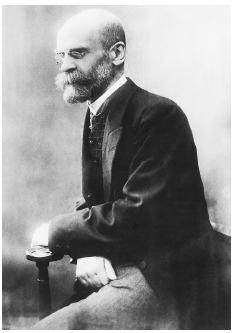
\includegraphics[scale=0.5]{images/durkheim}\\
	 \emph{(Épinal, Francia, 15 de abril 1858 — París, Francia, 15 de noviembre 1917)}\\
\end{center}
Uno de los fundadores de la sociología moderna, junto a Max Weber y Karl Marx.
Fundador de la primera revista dedicada a las ciencias sociales, el \emph{Année Sociologique},
con el cual también se identifica al grupo de estudiosos que desarrolló su programa de investigación sociológica.\\

Nació en Épinal, Francia, el 15 de abril 1858 en la región de Lorena.
A pesar de ser hijo de una familia profundamente religiosa (era hijo de un rabino),Durkheim tuvo una vida completamente secular.

Desde joven se sintió atraído por el método científico, que se oponía a su educación basada en la religión.

En muchos de sus trabajos, de hecho, estuvo dedicado a demostrar que los fenómenos religiosos provienen de factores sociales más que divinos.

Sus antecedentes judíos, sin embargo, moldearon su sociología, y muchos de sus estudiantes y colaboradores fueron compañeros judíos o parientes de sangre.

Durkheim entró a la École Normale Supérieure (Escuela Normal Superior), en 1879.
Su generación fue una de las más brillantes del siglo XIX y muchos de sus compañeros de clase, tales como Jean Jaurès y Henri Bergson se convertirían en importantes figuras de la vida intelectual francesa.

En la ENS (Escuela Normal Superior), Durkheim estudió con Fustel de Coulanges de su generación cuando se graduó en filosofía en 1882.
En 1887, es nombrado profesor de pedagogía y ciencia social de la Universidad de Burdeos.
Comienza con sus enseñanzas en sociología y fue el primero en enseñar esta ciencia en Francia.
Como consecuencia de los pesares que le causó la muerte de su único hijo, murió en París el 15 de noviembre de 1917.


\newpage


%inicio desarrollo

\section{Desarrollo}
\subsection{Obras}
\label{sec:obras}
El conjunto de trabajos de su obra la podemos resumir en siete puntos básicos:
\subsubsection{La solidaridad social}
		``La División del Trabajo Social'' (editada en 1893) fue su primer trabajo importante.
		La misma nació como la tesis doctoral con la que se recibió: ``La Solidaridad Social''.
		En ella intenta explicar la sociedad moderna mediante la división del trabajo y el derecho
		represivo por un lado, y por otro establece la crítica de la misma estableciendo la relación
		deseable entre el conocimiento positivo y el juicio normativo.
\subsubsection{El afincamiento de la sociología como ciencia autónoma}
		En dicho tópico sus obras fundamentales son: ``Las Reglas del Método Sociológico'' (1895) y ``El Suicidio'' (1897).
		En la primera define los principios epistemológicos de una ciencia positiva capaz de abordar al conocimiento
		concreto de las sociedades humanas, en forma totalmente independiente de las demás ciencias, esto es la sociología
		como ciencia autónoma; cosa que aún no habían podido definir ni Comte ni Spencer.
		En el segundo, realiza un estudio sociológico donde demuestra que lo que aparenta ser un hecho individual no es otra
		cosa que un hecho social, donde se relaciona la dependencia del individuo a factores externos y colectivos como son
		la religión, la economía y la familia.-
\subsubsection{Educación y pedagogía}
		Su artículo ``Educación'' publicado en el Nuevo Diccionario de Pedagogía y de Instrucción Primaria (1911),
		constituye un resumen de su pensamiento pedagógico. También dictó cursos en su cátedra sobre educación moral,
		historia de la pedagogía, éstos en las universidades de Burdeos y en la de París.
\subsubsection{Teoría política y derecho}
		Parte de la filosofía económica, jurídica y política del siglo XVIII y en base al estudio que hiciera de la obra
		de Saint Simón toma una posición eminentemente crítica respecto a las corrientes socialista y comunista.\\
		En la ``Física de las Costumbres y del Derecho'' (obra póstuma editada en 1950), compilación de sus cursos dictados,
		se divide el tema en dos partes: las solidaridades del grupo (la moral profesional y la moral cívica) y las solidaridades
		universales (donde trata sobre el respeto a la vida y al derecho de propiedad).
\subsubsection{La moral}
		Fue éste un tema recurrente en toda su obra:
		\begin{itemize}
			\item ``La Ciencia de la Moral en Alemania'' (1887)
			\item ``La Determinación del Hecho Moral'' (1906)
			\item ``Juicios de Valor y Juicios de Realidad'' (1911)
		\end{itemize}
		fueron los avances de la obra que no pudo editar en vida: ``Introducción a la Moral'';
		esta obra se canaliza en tres grandes temas:
		\begin{itemize}
			\item \textbf{a} concepto de la moral
			\item \textbf{b} el papel del moralista
			\item \textbf{c} desarrollo del concepto de una ciencia moral adecuada a sus tiempos.
		\end{itemize}
\subsubsection{La filosofía}
		Dada su formación filosófica, encara a la sociología con este perfil. Desarrolla una teoría sociológica de carácter
		ontológico en su obra ``Las Formas Elementales de la Vida Religiosa'' (1912).
\subsubsection{La religión}
		De su educación familiar en la tradición judía y su fe en la religión de la humanidad , se desprende la obra citada
		precedentemente en el item anterior.\\
		\emph{"La religión consiste en creencias y en prácticas relativas a las cosas sagradas".}\\
		Su concepto básico, en este tema, radica en comprender lo religioso en relación con lo sagrado sin necesidad de interponer
		los conceptos de la divinidad y el mas allá.
		Le importa demostrar que la experiencia religiosa no es exclusividad de sociedad alguna en particular, sino que por el
		contrario es un fenómeno universal.
		Entiende, por ser que históricamente todas las sociedades han experimentado un sentimiento religioso, que resulta
		imprescindible explicar la religión como un hecho social. La entiende como una experiencia real y no un acto imaginativo
		ya que es causa objetiva, universal y eterna de la religión de la humanidad.
		En resumen la misión de la ciencia social al respecto, es la de investigar el porqué de la causa de la religión como hecho
		social y no así el cuestionamiento de la religión en sí.
\newpage



\subsection{Pensamientos principales}
\label{sec:pensamiento}

\subsubsection{Los Hechos Sociales}
Sus antecesores tanto Comte como Spencer ve\'ian esta nueva ciencia con un profundo esp\'iritu positivista, d\'andole cualidades meramente organicistas o psicol\'ogicas, en tanto Durkheim epistemol\'ogicamente la independiz\'o de las restantes disciplinas cient\'ificas existentes.
 Es entonces que interpreta la existencia de fen\'omenos espec\'ificamente sociales a los que llam\'a ``hechos sociales'', que constituyen unidades de estudio que no pueden ser abordados con otras t\'ecnicas que no sean las espec\'ificamente sociales.\\
Durkheim define a los hechos sociales como: ``modos de actuar, de pensar y de sentir exteriores al individuo, y que poseen un poder de coerci\'on en virtud del cual se imponen''.\\

Las caracter\'isticas b\'asicas que representan a los hechos sociales son:
\begin{itemize}
	\item Exterioridad
	\item Coerci\'on
	\item Colectividad
\end{itemize}

Los hechos sociales existen con anterioridad al nacimiento de un individuo en determinada sociedad, por lo tanto son exteriores a \'el.\\
Por formar parte de la cultura de una sociedad son colectivos.\\
Y siendo que un individuo es educado conforme a las normas y reglas que rigen la sociedad donde naci\'o, son coercitivos.\\
Durkheim mismo ejemplifica hechos sociales genuinos diciendo: ``... si exist\'ian antes es que existen fuera de nosotros. El sistema de signos que utilizo para expresar mi pensamiento (lengua materna), el sistema monetario que empleo para pagar mis deudas, ...''\\
Analizando estos ejemplos llegamos a la conclusi\'on que todo rol que desempe\~namos en nuestra relaci\'on con los dem\'as seres humanos est\'an comprendidos dentro de un hecho social.\\

Sobre la coerci\'on, vale hacer una lectura de lo que el mismo dice: ```...Estos tipos de conducta o de pensamiento no son s\'olo exteriores al individuo, sino que est\'an dotados de un poder imperativo y coercitivo en virtud del cual se imponen a \'el, lo quiera o no.- ``... La conciencia pública reprime todo acto que la ofende''\\
``...Si yo no me someto a las convenciones del mundo, si al vestirme no tengo en cuenta los usos vigentes dentro de mi país y de mi clase, la risa que provoco, el alejamiento en que se me mantiene, producen, aunque en forma mas atenuada, los mismos efectos que un castigo propiamente dicho.''\\
Sobre la característica de la colectividad sigue diciendo: ``...Lo que los constituye son las creencias, las tendencias, las prácticas del grupo considerado colectivamente''. A título de ejemplo basta citar las normas parentales del antiguo pueblo judío que exigía ante la viudez de una cuñada, que el cuñado estaba comprometido a tomarla como esposa, también, y la protegería; iguales ejemplos son los diferentes conceptos actuales de diversas sociedades en torno a la relación marital, o bien a la primacía de un sexo sobre el otro en el contexto y comportamiento social.\\
Los hechos sociales tienen otra condición no menos importante que las anteriores y que es la de encarnarse en la psiquis de cada individuo de una sociedad y por tanto transformar la forma subjetiva de sentir determinados hechos o situaciones, por esta misma razón adquieren un carácter sui géneris, con valor en sí mismo y no como resultado de otros hechos sociales.\\
Esta forma de sentir cuando el hecho se presenta frente a la presencia de un grupo puede dar lugar a otro fenómeno social, el que pasamos a describir.\\

\subsubsection{Las Corrientes Sociales}
En la obra anteriormente mencionada, Durkheim los describe de la siguiente manera: ``...Así en una asamblea, los grandes movimientos de entusiasmo, de indignación, de piedad que se producen, no tienen como lugar de origen ninguna conciencia particular. Nos llegan a cada uno de nosotros desde fuera y son susceptibles de arrastrarnos a pesar nuestro. …Si un individuo intenta oponerse a una de esas manifestaciones colectivas, los sentimientos que rechazan se vuelven en su contra.''\\
Estas situaciones suelen ser de carácter emocional y por tanto breves, en algunas condiciones toman un giro racional, transformando así su permanencia, con lo que pueden volverse duraderas. Esto se puede demostrar por las diferentes etapas históricas por la que pasa un país cuando es marcado por un hito particular, por ejemplo el nacimiento de los partidos políticos tradicionales en el Uruguay.\\

\subsubsection{La divisi\'on del Trabajo Social}
Para esta obra Durkheim parte de la base del concepto de solidaridad.\\
Opone la organización de las sociedades arcaicas frente a la moderna y en relación con el espacio productivo que posean para su desarrollo.\\
En las sociedades pequeñas numéricamente y con amplia extensión productiva, la división del trabajo es casi imperceptible. A modo de ejemplo, en las civilizaciones neolíticas la caza era una función masculina, mientras que el laboreo de la tierra era de carácter femenino.\\
Estas sociedades por estar constituidas por segmentos sociales iguales les da el carácter de ``segmentado'' y en ellas existe un principio de ``solidaridad mecánica''.\\
Como consecuencia la solidaridad de la colectividad es muy estrecha por lo que la conciencia colectiva prácticamente anula a la individual. En estas sociedades, incluso la religión es unificadora.\\
Por el contrario en la medida que la sociedad crece numéricamente se hace imprescindible la diversificación del trabajo para poder atender las necesidades de la colectividad.\\
Esta diversificación laboral estratifica a la sociedad acorde a sus funciones, y en este sistema se establece lo que Durkheim da en llamar una ``solidaridad orgánica''.\\
Por el hecho que en las sociedades organizadas los individuos desarrollan diferentes aptitudes, aquellos que se concentran en un mismo tipo de funciones desarrollan diferentes enfoques de pensamiento, de estética, de ética, etc., por lo que la conciencia individual de un grupo se diferencia de los otros, y a su vez lo mismo ocurre con el individualismo dentro de cada subgrupo social.\\
Ante esta situación de crecimiento social, Durkheim, establece el concepto de ``densidad moral'' o ``dinámica''.\\
Dice: ``...cuanto mas numerosos son (los individuos) y cuanto más intensa es la acción de unos sobre otros, tanto más reaccionan con fuerza y rapidez y por consiguiente, tanto más intensa es la vida social''.\\
Con lo que la diversificación del trabajo es la solución encontrada, por él, ante la escasez, producto del crecimiento demográfico en un mismo espacio.\\
Mas adelante profundizará: ``...La división del trabajo varía en razón directa al volumen y a la densidad de las sociedades, …''.\\
Resumiendo, Durkheim especifica únicamente, que el crecimiento demográfico es la causa de todos los demás cambios sociales, por lo que su teoría en este tópico, ha sido clasificada como ``reduccionista''.\\
Sin embargo, en función del análisis que él hace sobre las sociedades de China y Rusia de su época, daría a entender que el crecimiento demográfico sería la causa de una mayor ''densidad dinámica``\\

\subsubsection{Educaci\'on}
Durkheim tambi\'en estaba interesado en la educaci\'on.

 Esto fue en parte porque trabajaba profesionalmente como capacitador de docentes, y \'el utiliz\'o su capacidad para afinar su curriculum para alcanzar sus metas de ense\~nar sociolog\'ia y expandirla como ciencia propia.

En t\'erminos m\'as generales, sin embargo, Durkheim estaba interesado en la forma en que la educaci\'on podr\'ia ser usada para proporcionar a los ciudadanos franceses la clase de contexto de solidaridad y secularidad necesaria para prevenir la anomia en la sociedad moderna.

Es en este sentido que tambi\'en propuso la formaci\'on de grupos de profesionales para servir como una fuente de solidaridad para los adultos. \\

Durkheim sostuvo que la educaci\'on tiene muchas funciones:

\begin{enumerate}
	\item Mejorar la solidaridad social
	\begin{itemize}
		\item Historia: Aprender sobre como las personas que han hecho buenas obras por los dem\'as hace sentir insignificante al individuo. 
	 	
% pledging -> ''promesas de contribuciones'', nose bien como traducirla, lo deje como:
          	\item Lealtad: Hace que las personas se sientan parte de un grupo y, por tanto, tiendan a haber menos posibilidades de que rompan las reglas.
	\end{itemize}
	\item Mantener el orden social
	\begin{itemize}
		\item La escuela es una sociedad en miniatura. Tiene una jerarquizaci\'on, reglas y espectaciones similares al del ``mundo exterior''. \'Esta entrena a la gente joven para que cumpla sus roles.
	\end{itemize}
	\item Mantener la divisi\'on del trabajo
	\begin{itemize}
		\item La escuela ordena a los estudiantes por grupos segun sus habilidades, animandolos a que elijan trabajos seg\'un las habilidades de cada uno.
	\end{itemize}
\end{enumerate}

\subsubsection{Crimen}
Durkheim ve\'ia que el crimen era el abandono de las nociones convencionales.
\'El creia que el crimen estaba ``ligado a las condiciones fundamentales de toda vida social'' y cumple una funci\'on en la sociedad.
\'El dictaba que el crimen era ``un util preludio para las reformas''.\\
En este sentido, vio al crimen capas de soltar ciertas tensiones sociales, teniendo un efecto purificador en la sociedad.
Llendo m\'as all\'a, estato que la autoridad que la conciencia moral disfrute no debe ser excesiva, ya que nadie se atrever\'ia a criticarla, provocando f\'acilmente un estado de forma inmutable.
Para que el progreso exista, la originalidad debe ser capaz de expresarse a s\'i misma, por lo que la originalidad del criminal tambi\'en debiera posibilitarse.

\subsubsection{Ley}
M\'as alla del estudio espec\'ifico de la ley, el crimen y el orden, Durkheim estaba profundamente interesado en el estudio de la ley y sus efectos sociales en general.
Entre los teoricos de la sociolog\'ia cl\'asica, el es uno de los fundadores de la socilogia de la ley.\\
En sus trabajos, el vio tipos de leyes, distingidas como represivas versus restitutivas (caracterizadas por sus sanciones), como reflejo directo de los tipos de la solidaridad social.
Por ello, el estudio de la ley fue de interes a la socilog\'ia por el hecho de poder revelar detalles sobre la naturaleza de la solidaridad.
Sin embargo, luego, \'el enfatiz\'o la importancia de la ley en s\'i como campo de estudio de la sociolog\'ia.
M\'as tarde, la visi\'on Durkheimiana vio a la ley (civil y criminal) como una expresi\'on que garantizaba los valores fundamentales de la sociedad.
Durkheim empatiz\'o con la forma en que la ley moderna crecientemente expresa una forma moral individualista - un sistema de valores que es, desde su punto de vista, probablemente el \'unico universalmente apropiadado a las condiciones modernas de la solidaridad social.
Individualismo, en este sentido, es la base de los derechos humanos y los valores de la dignidad individual humana y su individualidad autonoma.
Es duramente distingida de la avaricia y el egoismo, los cuales para Durkheim no son en lo absoluto posturas morales.\\
Muchos de sus seguidores m\'as cercanos, como Marcel Mauss, Georges Davy, Paul Fauconnet, Paul Huvelin, Emmanuel Levy y Henri Levy-Bruhl tambi\'en se especializaron o contribulleron al estudio de ley en la sociolog\'ia.

\subsubsection{El Suicidio}
En ``Suicide'' (1897), Durkheim explora las diferentes tasas de suicidios entre Protestantes y Cat\'olicos, concluyento que el mayor control social entre los Cat\'olicos resultaba en menores tasas de suicidio.
De acuerdo con Durkheim, la socidad Cat\'olica poseia niveles normales de integraci\'on social mientras que los Protestantes tenian niveles m\'as bajos.
Hay al menos dos problemas con \'esta interpretaci\'on.
Primero, Durkheim tom\'o la mayor\'ia de sus datos de investigadores anteriores, probablemente de Adolf Wagner y Henry Morselli, los cuales fueron mucho m\'as cuidadosos con la generalizaci\'on a partir de sus propios datos.  
Segundo, otros investigadores encontraron que las diferencias de las tasas de suicidios parecian estar limitadas a los Germano hablantes de Europa, por lo que podria haber sido el reflejo de otros factores.
A pesar de sus limitaciones, su trabajo en el suicidio a influenciado diferentes exponentes de la teor\'ia del control mencionados en el estudio de la sociolog\'ia cl\'asica.\\
Las conclusiones sobre el comportamiento individual son basados en las estadisticas de los suicidios. Este tipo de inferencias pueden ser a veces enga\~nosas, como son mostradas por los ejemplos dela paradoja de Simpson.\\

Durkheim dict\'o que habian cuatro tipos de suicidio.
\begin{description}
	\item[Suicidios Egoistas:]
		Son el resultado del debilitamiento de los lazos de integraci\'on de los individuos con la colectividad. En otras palabras, el quiebre de la integraci\'on social.\\
		Es la falla sintom\'atica del desarrollo econ\'omico y la divisi\'on del trabajo para producir la solidaridad organica de Durkheim.\\
		Su remedio esta en una recnostrucci\'on social.
	\item[Suicidios Altruistas:]
		Esto ocurre en sociedades con un alto nivel de integracion, donde las necesidades del individuo son menos importantes que las necesidades de la sociedad.\\
		Como el interes individual no es importante, Durkheim estima que en una sociedad altruista habrian pocas razones por las cuales las personas cometieran suicidio.\\
		Solo di\'o una exepci\'on: si el individuo espera que el suicidarse ayude a la sociedad.
	\item[Suicidios Animos:]
		Son el producto de la desregularizaci\'on moral y la falta de definiciones de aspiraciones leg\'itimas, dadas por una \'etica social restrictiva, la cual puede imponer orden y definir la conciencia individual.\\
		Es la falla sintom\'atica del desarrollo econ\'omico y la divisi\'on del trabajo para producir la solidaridad organica de Durkheim.\\
		Las personas desconocen donde ellos calzan dentro de su sociedad. \\
		Su remedio esta en una recnostrucci\'on social.
	\item[Suicidios Fatalistas:]
		Este tipo de suicidio parece ocurrrir en sociedades muy opresivas, causando que la gente prefiera morir que vivir dentro de la sociedad.\\
		Esta es una raz\'on extremadamente rara para que alguien se quite la vida, pero un buen ejemplo puede ser ir a prisi\'on; las personas pueden preferir la muerte que vivir en una prisi\'on con constantes abusos.
\end{description}

\subsubsection{Religi\'on}
En la socilog\'ia cl\'asica, el estudio de la religi\'on se concentraba principalmente en dos interrogantes:
\begin{enumerate}
	\item C\'omo la religi\'on contribuye a mantener un orden social? 
	\item Cual es la relaci\'on entre la religi\'on y la sociedad capitalista?
\end{enumerate}
Estas dos preguntas fueron t\'ipicamente combinadas con el argumento de que el capitalismo industrial cocavar\'ia los hechos religiosos tradicionales y por ello amenazar\'ia a la cohesi\'on de la sociedad.
Mas recientemente, el tema se a enfocado en el estudio de las instituciones religiosas. \\
En su art\'iculo,``El origen de las Creencias'' Durkheim se puso a si mismo en la tradici\'on positivista, significando que el pens\'o su estudio de la sociedad como desapasionado y cient\'ifico.
\'El estaba profundamente interesado en el problema que ten\'ian las sociedades modernas.
La religi\'on, argumentaba, era una expresi\'on de cohesi\'on social. \\

Sus intereses subyacentes eran el entender la existencia de una religi\'on en la ausencia de creencias de sus principios.
Durkheim veia el toteismo como la forma m\'as basica de religi\'on.
Es en este sistema de creencias en donde la separaci\'on entre lo sagrado y lo profano se ve claramente.
Todas las otras religiones, dice, son derivaciones de esta distinci\'on, agregandole mitos, iconos y tradiciones.
El animal tot\'emico, cre\'ia Durkheim, era la expresi\'on de lo sagrado y el foco original de la actividad religiosa a causa de que era el emblema del grupo social, del clan.
As\'i la religi\'on es inevitable, de igual forma como es inevitable que los individuas vivan juntos como grupo en una sociedad.\\

Durkheim penso que ese modelo para las relaciones entre las personas y lo sobrenatural fue la relaci\'on entre los individuos y la comunidad.
Pensaba que las personas ordenaban el mundo f\'isico, supernatural y el social acorde a principios similares.\\
Su primer prop\'osito era el identificar el origen social de la religi\'on, ya que la veia como una fuente de camaderias y solidaridad. 
Era una forma en que los individuos se volv\'ian reconocibles en frente de una sociedad establecida.
Su segundo proposito era el de identificar v\'inculo entre ciertas religiones en diferentes culturas, encontrando alg\'un denominador com\'un.
Creencias en realidades supernaturales y ocurrencias pueden no ser com\'un en todas las religiones, a\'un asi hay una clara divisi\'on entre diferentes aspectos de la vida, ciertos comportacmientos y cosas fi\'isicas.
En el pasado, argumentaba, la religi\'on habia sido el cimiento de la sociedad.
Sus definiciones de religi\'on, apoyadas por antrop\'ologos de hoy en d\'ia, era ``La religion es un sistema unificado de creencias y pr\'acticas relativas a cosas sagradas''.\\

Durkheim creia que la sociedad tenia que estar presente en el individuo.
Vi\'o en la religi\'on un mecanismo que fortalecia al orden social.
Pens\'o que la religi\'on hab\'ia sido un cimiento para la sociedad en el pasado, pero que el colapso de \'esta no llevar\'ia a una ``implosi\'on'' moral.
Durkheim estaba espec\'ificamente interesado en la religion como una experiencia de comunidad mas que una individual.
\'El incl\'uso dijo que el fen\'omeno religioso ocurria cuando se hacia una separaci\'on entre lo profano (la realidad de las actividades diarias) y lo sagrado (la realidad de los extraordinario y lo trascendental).
Un ejemplo de esto es la comuni\'on del vino, lo cual no es solo vino sino que representa la sangre de Jesucristo.
Adem\'as, en lugar de antepasados anteriores que intentaran reemplazar las religiones en decadencia, urg\'ian a las personas a unirse en una moralidad c\'ivica en las bases que ``somos lo que somos'' como resultado de la sociedad.\\

As\'i, Durkheim condenso las religiones en cuatro funciones mayores:
\begin{enumerate}
	\item Disciplinarias, forzando o administrando disciplina
	\item Cohesivas, juntando a las personas, generando fuertes lazos.
	\item Vitalizadoras, que aumentan el esp\'iritu, vitalizan y suben el \'animo.
	\item Euf\'oricas, con buenos sentimientos, felicidad, confidencia, bienestar.
\end{enumerate}
\newpage


\subsection{Cuestionario}
\label{sec:preguntas}
\begin{itemize}
	\item ?`Cu\'al es la teor\'ia o postulado m\'as importante del autor?\\
	El postulado m\'as importante de Durkheim es el de los ``hechos sociales'' en el cual identifica que existen hechos externos y anteriores a las personas
	que s\'olo pueden ser explicados desde el punto de vista de la sociedad en que \'estas viven. Con \'esto, Durkheim separ\'o el estudio de la sociedad de la rama 
	de la psicolog\'ia y form\'o la rama de sociolog\'ia moderna reconocida hasta hoy en d\'ia.

	\item ?`En qu\'e forma influye en las empresas (organizaciones) de su \'epoca y actualmente esta teor\'ia?\\
	Principalmente en la forma de afrontar ciertos fen\'omenos sociales, ya que \'estos anteriormente eran estudiados bas\'andose en los estudios de la psicolog\'ia.
	Gracias a la separaci\'on y las bases m\'as cient\'ificas utilizadas por Durkheim para describir y estudiar este tipo de fen\'omenos, es se han podido desarrollar
	las teor\'ias sobre las sociedades y como distintos factores de \'estas influyen positiva o negativamente en las personas que la conforman.

	\item ?`Qu\'e aspectos de la teor\'ia son dif\'iciles de comprender o aplicar?\\
	Sobre su teor\'ia de la ``solidaridad social'', un t\'ermino acu\~nado por Durkeim en el cual identifica un tipo de solidaridad en cada sociedad que influye en los 
	niveles de integraci\'on social de las personas, y induce un tipo de conciencia espec\'ifica a los individuos de cada comunidad. Al ser un t\'ermino usado para 
	explicar un ``comportamiento'' abstraido de los ``hechos sociales'' de la sociedad, es dif\'icil de comprender en un comienzo, pero no deja de ser un punto muy 
	importante en su teor\'ia sobre los fenomenos sociales. 

	\item ?`Qu\'e aspectos de la teor\'ia son criticados negativamente y cuales son alabados positivamente en la literatura? ?`Cu\'al es su posici\'on al respecto?\\
	De todos los estudios desarrollados por Durkheim, el \'unico que fue duramente criticado fue su trabajo sobre ``El Suicidio''. En \'este aspecto, sus concluciones sacadas del 
	estudio estad\'istico desarrollado (relacionando la mayor cantidad de suicidios en los de religi\'on Protestante en comparaci\'on con los de religi\'on Cat\'olica) 
	parecian estar limitadas a s\'olo el grupo estudiado, lo cual, hacia dudar de las generalizaciones realizadas en las concluciones alcanzadas por Durkheim. A pesar de ello,
	\'estos estudios han servido de inspiraci\'on para muchos pensadores y estudiosos de la Sociolog\'ia. Adem\'as, aunque uno pueda discutir el nivel de verdad de lo desarrollado 
	en lo respectivo a los suicidios, las conclusiones alcanzadas pueden extenderse y aplicarse de forma objetiva en otras situaciones sin muchas dificultades, por lo que 
	apoyamos a los conceptos e ideas obtenidas, a pesar de que el m\'etodo desarrollado para obtenerlas talvez no halla sido el m\'as adecuado.

	\item ?`Qu\'e lecciones aprende de su an\'alisis?\\
	La importancia de la sociolog\'ia en la sociedad moderna, partiendo de la base de que el an\'alisis de ciertos hechos o influencias en nuestra vida, como lo son,
	la religi\'on, el crimen, la educaci\'on, el suicidio, etc, pueden dar pie a una cierta estructura la cual seguimos, por ende gracias a las lecturas realizadas,
	nos pudimos dar cuenta como \emph{todo} factor externo, nos influencia a ser como somos, hasta el mas m\'inimo acto de algun cercano, va restringiendo nuestro
	actuar frente a cualquier fen\'onmeno. Todo depende de la sociedad, y para estudiar dichos fen\'omenos necesitamos s\'olo t\'ecnicas sociales, ning\'un otro
	mecanismo sirve.

	\item ?`C\'omo la vida personal del autor influy\'o en sus teor\'ias?\\
	Su vida en general, estuvo siempre ligada a la realidad de la comunidad judia en Francia, s\'olo un a\~no abandon\'o su pa\'is para ir a estudiar en Alemania, pero
	volvi\'o a la brevedad. Parti\'o sus estudios en Filosof\'ia e Historia y de a poco fue acerc\'andose a la Pscicolog\'ia, campo en el cual se di\'o cuenta de la
	importancia de la Sociolog\'ia, raz\'on por la cual deb\'ia ser una ciencia distinta. Junto a algunos colegas fundo una revista dedicada a su estudio la cual tuvo
	mucho \'exito, por ende su vida, estuvo siempre ligadas a sus estudios, ya que a medida que iba abarcando nuevos estudios iba haciendo nuevas investigaciones.
	Ya que se sent\'ia influenciado por el m\'etodo cient\'ifico, y ten\'ia algunas creencias cat\'olicas, pod\'ia realizar estudios abarcandolos de los dos puntos de
	vista, por ende su vida, y el ambiente de su crecimiento (reinado por el positivismo) fueron dando pauta a el esqueleto de sus estudios.

	\item ?`Qu\'e c\'odigo de conducta o creencias marcaron la forma de pensar del autor analizado?\\
	Durkheim proven\'ia de una familia judia, ocho generaciones de rabinos fueron con su padre y el quebr\'o dicha tradici\'on, ya que por influencias de un profesor de
	la universidad se convirtió al catolicismo. Por \'este motivo y pensando en que la gente criticaria su forma de actuar y de pensar aludiendo a un \emph{``es por sus
	tradiciones religiosas que posee dicha opini\'on''}, decidi\'o alejar sus pensamientos y trabajos lo m\'as posiblemente de la religi\'on y tratar de dejar de lado
	todo el espiritualismo y tradiciones. De todas formas en m\'as de alg\'un trabajo critica fuertemente la religiosidad, comparandola con una especie de sociedad primitiva y buscando similitudes entre los distintos tipos de creencias de las diferentes religiones.

	\item ?`Qu\'e valores o principios \'eticos muestran los escritos del autor analizado?\\
	Claramente, sus estudios le dan gran importancia a los principios del orden, la responsabilidad social y la solidaridad entre los miembros de una sociedad. Marcado de 
	una u otra forma por sus antecedentes religiosos, Durkheim fundo sus conceptos bajo la idea que la sociedad debe tender a un orden social que logre la integraci\'on de 
	sus miembros orientados hacia el bien com\'un de la comunidad. Estos principios son los principales por los cuales se rigen las llamadas ``sociedades primitivas'', tales 
	como los sistemas organizacionales de la Iglesia o el Ejercito. A\'un as\'i, logro destacar la importancia del valor \'etico-social del individualismo (lo cual no debe 
	confundirse con la avaricia y el egoismo, los cuales no son en lo absoluto considerados como posturas morales por Durkheim).
	Durkheim vi\'o al individualismo como la base de los derechos humanos y los valores de la dignidad individual humana y su individualidad aut\'onoma, siendo muy importantes 
	para el desarrollo de las sociedades modernas caracterizadas por solidaridad org\'anica.

\end{itemize}
\newpage


%fin desarrollo

\section{Conclusiones}
\label{sec:conclusiones}
\subsection{Conclusiones Individuales}
%Conclusiones personales
Personalmente pude comprender la importancia de la sociedad en un individuo, sobre todo cuando Durkheim se refiere a que el suicidio es un hecho social y no un hecho individual,
la culpa no es del sujeto, es de la sociedad.

Otro aspecto importante es como la sociedad nos ense\~na a actuar, a pensar, todo respecto a sus mismos est\'andares, y la sociedad castiga muy duramente a quien no act\'ua como
ella misma le ense\~no, un aspecto muy claro que se puede apreciar mirando una cultura determinada, el extremismo y como muchas personas viven con sus ojos vendados, aceptando
una verdad local, que a los ojos del resto del mundo puede estar erroneo, pero ?`No es el resto del mundo otra macro-cultura que también nos obliga a pensar de una forma?

Principalmente, pude darme cuenta que la visi\'on que ten\'ia Durkheim con respecto a la sociedad, fue una marca intachable en la historia del pensamiento humano,
ya que el separandose de todos los aspectos posibles, dejando atr\'as emociones, prejuicios, creencias, pudo generar un juicio imparcial para poder formar o declarar
la sociolog\'ia actual como una ciencia, que hoy en d\'ia es una de las ciencias mas importantes para el estudio de la humanidad

Finalmente, a nivel  personal me llamo mucho la atenci\'on como pudo tener la valent\'ia en su tiempo de poder analizar fen\'omenos sociales, sin ninguna influencia tan notoria
dejando de lado pensamiento que ven\'ian de 8 generaciones antes que el a nivel familiar, y que si nos damos cuenta claramente son la estructura de la organizaci\'on llamada sociedad.
Sin dejar de lado, la capacidad que tuvo para poder describir que una organizaci\'on se puede llevar a la autodestrucci\'on (Anomia), t\'ermino que sirvi\'o y sirve notablemente al
momento de analizar los riesgos de las organizaciones actuales.



\subsection{Conclusiones Generales}
%Conclusiones 'en conjunto' ......

La visi\'on de Durkheim de la sociedad marc\'o al pensamiento mundial en una manera que era
muy necesaria, dejar de lado todo tipo de prejuicios y emociones para generar un juicio imparcial y
racional de \'esta se volvio el pilar de la Sociolog\'ia, ciencia que hoy en dia se ha establecido como
una de las mas importantes de las Ciencias Sociales.

A trav\'es de las ideas del autor, las empresas se pueden analizar con ``sangre fr\'ia'', extrapolan-
do las ideas de ``hechos sociales'' y ``estructura'' a organizaciones mas pequeñas. De esta manera se
puede entender mejor la forma de comportarse de algunas organizaciones que tienden
a la autodestrucci\'on o que logran surgir en ambientes altamente hostiles.

%	\item Sobre los hechos sociales
Adem\'as, cuando uno es insertado en una nueva comunidad, como lo es una organizaci\'on o empresa hoy en d\'ia, uno 
se ve rodeado de un sistema con una cultura propia y muchas veces diferente a la del individuo. Estos 
detalles impl\'icitos muchas veces dentro dela organizaci\'on, son los reconocidos como ``hechos sociales''
por Durkheim. Por ello, podemos concluir que fue importante que Durkheim halla reconocido que los 
hechos sociales deb\'ian ser analisados por m\'etodos diferentes a los de la psicolog\'ia, ya que los estudios 
de sociolog\'ia desarrollados por \'el han sido un gran aporte para el estudio de la administraci\'on general 
de estos ``sistemas humanos'', jugando un rol medular en el asunto. 

%	\item Sobre las Corrientes Sociales\\
Tambi\'en, esto dicho anteriormente  deber\'iamos encararlo con objetividad, desprendiéndonos de todos los prejuicios y preconceptos que podamos tener antes de abordarlos.\\
Esto puede llegar a ser muy difícil, si a modo de ejemplo tomamos por punto de partida que el analista pertenece a una colectividad, a una sociedad, que tiene determinado su pensamiento a través del lenguaje que determina en sí mismo una estructura preestablecida de pensamiento lógico.


%	\item Sobre la divisi\'on del trabajo social\\
Para el estudio y administraci\'on de empresas u organizaciones, el concepto de solidaridad desarrollado
por Durkheim es importante de recalcar. Vi\'endolo desde su punto de vista, cada organizaci\'on deber\'ia 
buscar una solidaridad mec\'anica entre sus miembros. De esta forma, los individuos lograr\'ian adquirir 
una mentalidad enfocada a los objetivos de la empresa (vista como comunidad), y as\'i, mantener un 
ambiente de unidad y confianza en torno a los ideales de \'esta. Es notable mencionar que muchas 
organizaciones tienden a de hoy en dia tienden a fomentar un ambiente competitivo entre sus integrantes, 
lo cual, al igual que la mentalidad individualista en la realidad actual, conlleva muchas veces a problemas 
t\'ipicos de una solidaridad org\'anica.

%	\item  Sobre la educaci\'on\\
Ahora si analizamos las las funciones de la educaci\'on destacadas por Durkheim, desde el punto de vista de las organizaciones, 
la educaci\'on sirve como herramienta para lograr un mayor orden social, una mayor lealtad y una mayor especializaci\'on 
de los integrantes hacia la comunidad, siendo as\'i de gran importancia para mejorar la integraci\'on de nuevos miembros
y el crecimiento de la empresa.
	
%	\item  Sobre el Crimen
%Durkheim identific\'o al crimen como un indicador de la necesidad de cambios dentro de las organizaciones. 

%	\item Sobre la Ley
%Postulados principales:
% Diferencia duramente entre el Individualismo y la avaricia y el egoismo
% Avaricia y egoismo no son en lo absoluto posturas morales
% Estudia la Ley como una expresi\'on que garantizaba los valores fundamentales de la sociedad.

%	\item Sobre el Suicidio\\
De la misma manera, Durkheim, con su trabajo sobre el suicidio de los individuos con diferentes hechos sociales, logra destacar como ciertos 
factores en la sociedad (debilitamiento de los lazos de integraci\'on, desregularizaci\'on moral y falta de definiciones 
leg\'itimas, sociedades muy opresivas) pueden llevar a la autodestrucci\'on de sus miembros.\\
Por ello, se puede concluir que  es importante que las organizaciones se preocupen de mantener a sus integrantes 
cuidando de no desarrollar estas fallas que requieren de una reconstrucci\'on social.

%	\item Sobre la Religi\'on\\
Por \'ultimo, sus estudios sobre la religi\'on permitieron comprender mejor el desarrollo del orden social en las primeras comunidades, 
cumpliendo estas la funci\'on de separar lo mundano o cotidiano de las cosas intangibles, que relacionadas con lo sagrado, 
lograban la generaci\'on de normas que fomentaban el orden social.



\newpage


\section{Referencias}
\label{sec:referencias}
\begin{itemize}
%	\item Wikipedia, the free encyclopedia 
	\item http://www.luventicus.org/articulos/03U011/durkheim.html
	\item http://usuarios.lycos.es/politicasnet/autores/durkheim.htm
	\item http://www.biografiasyvidas.com/biografia/d/durkheim.htm
	\item http://www.emile-durkheim.com/
	\item http://en.wikipedia.org/wiki/Émile\_Durkheim
	\item http://www.epdlp.com/escritor.php?id=1667
	\item http://durkheim.pais-global.com.ar/
	\item Definiciones: 	
	\begin{itemize}
			\item Google Translate
			\item http://es.thefreedictionary.com
			\item http://www.wordreference.com/es/ 
	\end{itemize}
\end{itemize}
\newpage


\section{Glosario}
\label{sec:glosario}
\begin{description}
	\item[Memoria Principal:]
Está formada por bloques de circuitos integrados o chips capaces de almacenar, retener o ``memorizar''
información digital, es decir, valores binarios; a dichos bloques tiene acceso el microprocesador de la
computadora. El microprocesador la accede mediante el bus de direcciones. La MP es el núcleo del
sub-sistema de memoria de un computador, y posee una menor capacidad de almacenamiento que la memoria
secundaria, pero una velocidad muy superior.

	\item[Bus:]
Es un sistema digital que transfiere datos entre los componentes de un computador o
entre computadores. Están formado por cables o pistas en un circuito impreso, dispositivos como
resistencias y condensadores además de circuitos integrados. La función del Bus es la de permitir la
conexión lógica entre distintos subsistemas de un sistema digital, enviando datos entre dispositivos de
distintos ordenes: desde dentro de los mismos circuitos integrados, hasta equipos digitales completos que
forman parte de supercomputadoras.

	\item[Memoria Caché:]
Es un sistema especial de almacenamiento de alta velocidad. Puede ser tanto un área reservada de la
memoria principal como un dispositivo de almacenamiento de alta velocidad independiente. Hay dos tipos de
cache frecuentemente usados en las computadoras personales: memoria cache y cache de disco. Una memoria
cache, llamada también a veces almacenamiento cache o RAM cache, es una parte de memoria RAM estática de
alta velocidad (SRAM) más que la lenta y barata RAM dinámica (DRAM) usada como memoria principal. La
memoria cache es efectiva dado que los programas acceden una y otra vez a los mismos datos o
instrucciones. Guardando esta información en SRAM, la computadora evita acceder a la lenta DRAM.

	\item[Principio de Localidad:]
Los programas acceden una porción relativamente pequeña del
espacio de direcciones en un determinado instante de tiempo.

	\item[Localidad Espacial:]
Se refiere al espacio en donde son guardados los datos en la memoria. Es una propiedad en la que se basa
una de las políticas de extracción utilizadas para determinar cuándo y qué bloque de memoria principal
hay que traer a memoria cache. Si un item es referenciado, los items tenderán a ser referenciados a la
brevedad.

	\item[Localidad Temporal:]
Se refiere a la frecuencia con la cual son consultados ciertos bloques guardados en la memoria.
Si un item es referenciado, tenderá a ser referenciado nuevamente a la brevedad.

	\item[Latencia:]
En redes informáticas de datos se denomina latencia a la suma de retardos temporales dentro de una red.
Un retardo es producido por la demora en la propagación y transmisión de paquetes dentro de la red.

	\item[Ciclos de Reloj:]
La frecuencia de reloj indica la velocidad a la que un ordenador realiza sus operaciones más básicas,
como sumar dos números o transferir el valor de un registro a otro. Se mide en ciclos por segundo
(hercios).
	\item[CPU:]
Es el componente en una computadora digital que interpreta las instrucciones y procesa los datos
contenidos en los programas de la computadora. Las CPU proporcionan la característica fundamental de la
computadora digital (la programabilidad) y son uno de los componentes necesarios encontrados en las
computadoras de cualquier tiempo, junto con el almacenamiento primario y los dispositivos de
entrada/salida. 
\end{description}


\end{document}
